\begin{back}{格点模型的一种数值计算方法——张量网络}{tensor-network}
    文献\cite{Orus_tensor}给出了对常用的张量网络的一些介绍。
    所谓\concept{张量网络}是指通过缩并一些张量得到的格点系统波函数(称为\concept{张量网络态})的试探形式。
    使用张量网络方法能够自然地引入对称性,能够很容易地从最终计算结果中获得诸如纠缠熵等信息,能够用于分析各种边界条件的系统,处理无穷系统比较方便,图形化语言意义清晰等等(例如对局域的哈密顿量,相邻格点的纠缠总是比较大,通过分析张量网络态中的纠缠我们能够确定一个模型的基态的“有效格点结构”)。
    相较于量子蒙卡方法,张量网络方法的不足之处则在于难以估计计算质量好坏。

    需要保证使用的张量网络态真的是足够好的拟设——选择一个张量网络波函数拟设本质上是在将系统的希尔伯特空间按照纠缠程度做分类,选择一个张量网络拟设等价于选择纠缠程度适当的一个子空间,如对有能隙系统,低能能量本征态的一个空间部分的纠缠熵正比于该空间部分的表面积(所谓\concept{area law}),因此我们应该选择一个服从area law的张量网络拟设。
    此外,高效地实施张量网络计算需要适当安排缩并顺序。设张量网络图中每条线代表的指标的取值范围大致在1到$d$(这个$d$称为这条边的维数,但是这个维数和晶格的维数、每个格点上的标签的取值数目(所谓“本地维数”)这三者之间没有必然联系),则计算一个有$n_1$条外线,$n_2$条内线的张量网络缩并的时间复杂度大致在$\bigO{d^{n_1+n_2}}$。
    例如,普通的矩阵乘法$[A_{ij} B_{jk}]_{ij}$涉及三条线——$i, j, k$——因此其时间复杂度为$\bigO{d^3}$。
    适当地安排缩并顺序可以大幅降低计算整体的时间复杂度。

    张量网络和图形演算(见\autoref{back:anyon-tensor-category})之间有比较紧密的关系,但是它们并不完全是一回事。如果说后者像是微分几何中的逆变、协变矢量,前者就像是矩阵论。
    一个很容易看出的区别是引脚位置:在图形演算中,有明确物理意义的量——量子态,算符等——的指标或者说引脚是分前后顺序的(因为需要区分逆变和协变),图形上,有的向左有的向右。
    张量网络中不存在这样的区分。不过,就像一个区分逆变协变的微分几何方程可以用一个只有矩阵运算的线性代数库做数值计算一样,一个图形演算中的图形原则上也总是可以画成张量网络——简单地将指标向左或是向右的意义忘掉,并且在适当的地方加一个复共轭即可。
    然而,一旦我们需要在某一组基矢量下展开态矢量等——这件事经常需要做,比如在我们谈论局域性的时候——没有更多结构的图形演算是很难用的。
    一个张量网络中很容易表示的MPS在一个没有附加结构的图形演算中要如何表示呢?
    不过这不是说两者在具体计算上没有任何关系。在一些数值计算问题中,我们需要自动地快速计算一些图形演算的图,如何将它们转化成特定基矢量下的、能够快速计算的张量网络图是非常非平凡的问题。
    还有一些时候张量网络无法展示图形演算中的结构,我们需要根据图形演算的一些数据来约束张量网络的形式。

    可能最有名的张量网络方法就是\concept{密度矩阵重整化群(DMRG)}了。这是一种主要用于分析一维格点系统的张量网络方法,其基态波函数拟设为\concept{矩阵乘积态(MPS)},绘制为\autoref{fig:mps-state}。
    要施加开放边界条件只需移除左右两条外线,要施加周期性边界条件只需要将左右两个外线连接起来。
    在\cite{Orus_tensor}中介绍了MPS的一些性质:可以做到平移不变(只需让每个蓝点指向同一个张量即可),稠密(只要$d$足够大原则上可以构造出任意的一维格子上的波函数),纠缠熵服从area law,关联长度受控制等等。
    DMRG获得这个名字是因为MPS实际上是一种实空间重整化群(也称为DMRG)产生的基态波函数——实空间重整化群的主要难题在于,$N$格点哈密顿量的最低几个能量本征态未必和$N+1$格点哈密顿量的最低几个能量本征态有足够大的重叠,从而朴素地“保留能量最低的几个能量本征态——加入新格点——对角化”的方法通常精度严重不足。
    DMRG重整化群根据约化密度矩阵来保留能量本征态,从而可以考虑到新加入格点和已有格点之间的量子纠缠信息,这就是它的名字的由来。

    实空间重整化群由于种种问题(如根本不知道应该保留什么样的能量本征态),发展困难,而DMRG的张量网络形式却获得了快速发展,并成功地推广到更高维系统中。
\end{back}

\begin{figure}
    \centering
    

\tikzset{every picture/.style={line width=0.75pt}} %set default line width to 0.75pt        

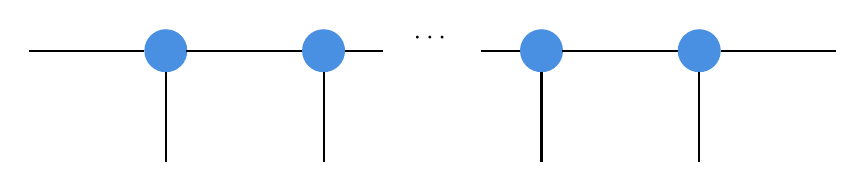
\begin{tikzpicture}[x=0.75pt,y=0.75pt,yscale=-1,xscale=1]
%uncomment if require: \path (0,300); %set diagram left start at 0, and has height of 300

%Straight Lines [id:da3529828319821786] 
\draw    (100,121) -- (155.71,121) ;
%Shape: Circle [id:dp4966257648856902] 
\draw  [draw opacity=0][fill={rgb, 255:red, 74; green, 144; blue, 226 }  ,fill opacity=1 ] (155.71,121) .. controls (155.71,115.28) and (160.34,110.65) .. (166.06,110.65) .. controls (171.78,110.65) and (176.41,115.28) .. (176.41,121) .. controls (176.41,126.72) and (171.78,131.35) .. (166.06,131.35) .. controls (160.34,131.35) and (155.71,126.72) .. (155.71,121) -- cycle ;
%Straight Lines [id:da5097517964421374] 
\draw    (166.06,131.35) -- (166.06,174.47) ;
%Straight Lines [id:da5757875200950937] 
\draw    (176,121) -- (231.71,121) ;
%Shape: Circle [id:dp31753487336843933] 
\draw  [draw opacity=0][fill={rgb, 255:red, 74; green, 144; blue, 226 }  ,fill opacity=1 ] (231.71,121) .. controls (231.71,115.28) and (236.34,110.65) .. (242.06,110.65) .. controls (247.78,110.65) and (252.41,115.28) .. (252.41,121) .. controls (252.41,126.72) and (247.78,131.35) .. (242.06,131.35) .. controls (236.34,131.35) and (231.71,126.72) .. (231.71,121) -- cycle ;
%Straight Lines [id:da5499396691584562] 
\draw    (242.06,131.35) -- (242.06,174.47) ;
%Shape: Circle [id:dp46956631085551503] 
\draw  [draw opacity=0][fill={rgb, 255:red, 74; green, 144; blue, 226 }  ,fill opacity=1 ] (336.71,121) .. controls (336.71,115.28) and (341.34,110.65) .. (347.06,110.65) .. controls (352.78,110.65) and (357.41,115.28) .. (357.41,121) .. controls (357.41,126.72) and (352.78,131.35) .. (347.06,131.35) .. controls (341.34,131.35) and (336.71,126.72) .. (336.71,121) -- cycle ;
%Straight Lines [id:da05730224870138678] 
\draw    (347.06,131.35) -- (347.06,174.47) ;
%Straight Lines [id:da830776528549658] 
\draw    (357,121) -- (412.71,121) ;
%Shape: Circle [id:dp008803468324955599] 
\draw  [draw opacity=0][fill={rgb, 255:red, 74; green, 144; blue, 226 }  ,fill opacity=1 ] (412.71,121) .. controls (412.71,115.28) and (417.34,110.65) .. (423.06,110.65) .. controls (428.78,110.65) and (433.41,115.28) .. (433.41,121) .. controls (433.41,126.72) and (428.78,131.35) .. (423.06,131.35) .. controls (417.34,131.35) and (412.71,126.72) .. (412.71,121) -- cycle ;
%Straight Lines [id:da019733050780630812] 
\draw    (423.06,131.35) -- (423.06,174.47) ;
%Straight Lines [id:da7512416171551617] 
\draw    (433.41,121) -- (489.12,121) ;
%Straight Lines [id:da28870663678175323] 
\draw    (252.41,121) -- (270.71,121) ;
%Straight Lines [id:da6449842400542742] 
\draw    (317.71,121) -- (336.71,121) ;

% Text Node
\draw (284,110.4) node [anchor=north west][inner sep=0.75pt]    {$\cdots $};


\end{tikzpicture}

    \caption{MPS拟设,根据不同的边界条件可以调整最左边和最右边两个外线;向下的线连接每个格点上的基矢量}
    \label{fig:mps-state}
\end{figure}